\section{Cardinality, Choice, and Infinite Sets}

Choice and maximality principles come first as foundational tools; cardinality then compares sets by functions rather than by informal size.

\subsection{Choice and Zorn's Lemma}

\begin{definition} \label{def:choice-function} \hlt{Choice Function}\\
Let $\mathcal{F}$ be a family of nonempty sets, let $I$ be a set, and let $(X_i)_{i\in I}$ be an indexed family of nonempty sets.
\begin{enumerate}[label=(\roman*)]
\setlength{\itemsep}{0pt}
\item A \hlt{choice function} on $\mathcal{F}$ is a map $c:\mathcal{F}\to\bigcup\limits_{F\in\mathcal{F}}F$ satisfying $(\forall F\in\mathcal{F})\,c(F)\in F$.
\item An \hlt{indexed choice function} for $(X_i)_{i\in I}$ is a map $c:I\to\bigcup\limits_{i\in I}X_i$ satisfying $(\forall i\in I)\,c(i)\in X_i$.
\end{enumerate}
\end{definition}

\begin{principle} \label{princ:axiom-of-choice-analysis} \hlt{Choice Principle}\\
Let $I$ be a set and let $(X_i)_{i\in I}$ be an indexed family of nonempty sets. The axiom of choice asserts $(\exists c:I\to\bigcup\limits_{i\in I}X_i)(\forall i\in I)\,c(i)\in X_i$.\\
Equivalently, $\prod\limits_{i\in I}X_i\neq\varnothing$. An explicit $c$ proves existence directly; the principle supplies simultaneous choices without an explicit rule.
\end{principle}

\begin{principle} \label{princ:zorns-lemma} \hlt{Zorn's Lemma}\\
Let $(P,\leq)$ be a poset with $P\neq\varnothing$. Assume the following chain-upper-bound condition.\\
$(\forall C\subseteq P)\,[((\forall x,y\in C)\,(x\leq y\lor y\leq x))\Rightarrow(\exists u\in P)(\forall c\in C)\,c\leq u]$. Then $(\exists m\in P)(\forall x\in P)\,(m\leq x\Rightarrow x=m)$.
\end{principle}

\begin{definition} \label{def:inclusion-and-containment-orders-for-zorn} \hlt{Inclusion and Containment Orders}\\
Let $\mathcal{F}$ be a family of sets and let $\mathcal{A}\subseteq\mathcal{F}$.
\begin{enumerate}[label=(\roman*)]
\setlength{\itemsep}{0pt}
\item \hlt{Inclusion}: for $A,B\in\mathcal{F}$, define $A\leq B$ iff $A\subseteq B$. An upper bound of $\mathcal{A}$ is $U\in\mathcal{F}$ satisfying $(\forall A\in\mathcal{A})\,A\subseteq U$.\\
An element $M\in\mathcal{F}$ is maximal iff $(\forall B\in\mathcal{F})\,(M\subseteq B\Rightarrow B=M)$.
\item \hlt{Reverse inclusion}: for $A,B\in\mathcal{F}$, define $A\leq B$ iff $B\subseteq A$. An upper bound of $\mathcal{A}$ is $U\in\mathcal{F}$ satisfying $(\forall A\in\mathcal{A})\,U\subseteq A$.\\
An element $M\in\mathcal{F}$ is maximal iff $(\forall B\in\mathcal{F})\,(B\subseteq M\Rightarrow B=M)$.
\end{enumerate}
\end{definition}

\begin{proposition} \label{prop:inclusion-and-reverse-inclusion-partial-orders} \hlt{Inclusion Orders Are Partial Orders}\\
Let $\mathcal{F}$ be a family of sets. Inclusion and reverse inclusion are partial orders on $\mathcal{F}$.
\begin{proof}
Fix $A,B,C\in\mathcal{F}$. Since $A\subseteq A$, inclusion is reflexive. If $A\subseteq B$ and $B\subseteq C$, then $A\subseteq C$, so inclusion is transitive.\\
If $A\subseteq B$ and $B\subseteq A$, then $A=B$ by Assumption \ref{assump:set-extensionality}, so inclusion is antisymmetric. Hence inclusion is a partial order.\\
For reverse inclusion, $A\supseteq A$ gives reflexivity, $A\supseteq B\supseteq C$ gives $A\supseteq C$, and $A\supseteq B\supseteq A$ gives $A=B$ by Assumption \ref{assump:set-extensionality}.\\
Thus reverse inclusion is also a partial order.\\
\hlt{Structural Commentary}: Each order law follows from the corresponding containment law and set extensionality.\\
\hlt{Key Insight}: Reversing containment preserves reflexivity, transitivity, and antisymmetry.
\end{proof}
\end{proposition}

\begin{proofmethod} \label{meth:zorn-maximality-template} \hlt{Zorn Maximality Template}\\
Use this method when the target follows from a candidate admitting no proper admissible extension.\\
Let $P$ be the set of candidates, and let $\leq$ record admissible extension.
\begin{enumerate}[label=(\roman*)]
\setlength{\itemsep}{0pt}
\item Verify that $P\neq\varnothing$ and that $\leq$ is a partial order on $P$.
\item Fix a chain $C\subseteq P$, construct $u\in P$, and prove $(\forall p\in C)\,p\leq u$.
\item Obtain a maximal $m\in P$ by Principle \ref{princ:zorns-lemma}, and prove that maximality forces the target property.
\end{enumerate}
For $C\neq\varnothing$, common candidates are $\bigcup\limits_{A\in C}A$ under inclusion and $\bigcap\limits_{A\in C}A$ under reverse inclusion.\\
Under reverse inclusion, another object contained in every member of $C$ may be necessary.\\
If $C=\varnothing$, any element of $P$ is an upper bound. In every case, prove $u\in P$; this is the indispensable admissibility check.\\
\hlt{Key Idea}: A chain bound must preserve every admissibility condition defining the candidate set.
\end{proofmethod}


\subsection{Same Cardinality, Finite, Countable, and Uncountable}

\begin{definition} \label{def:cardinality-equivalence} \hlt{Same Cardinality}\\
For sets $A,B$, define $A\sim_{\#}B$ iff there exists a bijection $f:A\to B$.\\
Then $A$ and $B$ have \hlt{same cardinality}, or are \hlt{equivalent}. The relation $\sim_{\#}$ is an equivalence relation.\\
$\operatorname{id}_A$ proves reflexivity, inverses of bijections prove symmetry, and composition of bijections proves transitivity.
\end{definition}

\begin{definition} \label{def:finite-countable-uncountable} \hlt{Finite, Countable, and Uncountable}\\
Set $J_0\defeq\emptyset$, and for $n\geq1$ set $J_n\defeq\{1,2,\ldots,n\}$. A set $A$ is
\begin{enumerate}[label=(\roman*)]
\setlength{\itemsep}{0pt}
\item \hlt{finite} if $A\sim_{\#} J_n$ for some $n\in\N$;
\item \hlt{infinite} if it is not finite;
\item \hlt{countable} if $A\sim_{\#} \N$;
\item \hlt{uncountable} if it is neither finite nor countable;
\item \hlt{at most countable} if it is finite or countable.
\end{enumerate}
Countable sets are also called enumerable or denumerable.
\end{definition}

\begin{proposition} \label{prop:finite-cardinality-well-defined} \hlt{Finite Cardinality is Well Defined}\\
Let $m,n\in\N$. If $A\sim_{\#}J_m$ and $A\sim_{\#}J_n$, then $m=n$.\\
Hence for finite $A$, the value $\#A\defeq n$ with $A\sim_{\#}J_n$ is well-defined.
\begin{proof} By transitivity of $\sim_{\#}$, it suffices to prove $J_m\sim_{\#}J_n\Rightarrow m=n$.\\
Induct on $m$. If $m=0$, then $J_m=\emptyset$, so any bijection $J_m\to J_n$ forces $J_n=\emptyset$ and $n=0$.\\
Assume the claim for $m-1$, with $m\geq1$, and let $f:J_m\to J_n$ be bijective. Then $n\geq1$.\\
Removing $m$ and $f(m)$ gives a bijection $J_m\setminus\{m\}\to J_n\setminus\{f(m)\}$. Since these sets have the standard relabelings $J_{m-1}$ and $J_{n-1}$, the induction hypothesis gives $m-1=n-1$, hence $m=n$.\\
\hlt{Structural Commentary}: Finite size is bijection-invariant.\\
\hlt{Key Insight}: Remove one matched element.
\end{proof}
\end{proposition}

\begin{definition} \label{def:finite-set-summation} \hlt{Summation over a Finite Set}\\
Let $X$ be a finite set with $\#X=n$, and let $f:X\to\C$.\\
Choose any bijection $g:J_n\to X$, where $J_n=\{1,\ldots,n\}$, and set $\sum\limits_{x\in X}f(x)\defeq\sum_{i=1}^{n}f(g(i))$.\\
When $X=\emptyset$, this is the empty sum $0$.\\
\hlt{Key Insight}: Proposition \ref{prop:finite-set-summation-laws} shows that the value is independent of the chosen bijection.
\end{definition}

\begin{proposition} \label{prop:finite-set-summation-laws} \hlt{Finite Set Summation Laws}\\
Let $X,Y$ be finite sets.
\begin{enumerate}[label=(\roman*)]
\setlength{\itemsep}{0pt}
\item \hlt{Well-definedness}: different bijections $J_{\#X}\to X$ give the same value in Definition \ref{def:finite-set-summation}.
\item \hlt{Substitution}: if $h:Y\to X$ is a bijection and $f:X\to\C$, then $\sum\limits_{x\in X}f(x)=\sum\limits_{y\in Y}f(h(y))$.
\item \hlt{Linearity}: for $f,g:X\to\C$ and $c\in\C$, $\sum\limits_{x\in X}(f(x)+g(x))=\sum\limits_{x\in X}f(x)+\sum\limits_{x\in X}g(x)$ and $\sum\limits_{x\in X}cf(x)=c\sum\limits_{x\in X}f(x)$.
\item \hlt{Disjoint unions}: if $X\cap Y=\emptyset$ and $f:X\cup Y\to\C$, then $\sum\limits_{z\in X\cup Y}f(z)=\sum\limits_{x\in X}f(x)+\sum\limits_{y\in Y}f(y)$.
\item \hlt{Finite Fubini}: if $f:X\times Y\to\C$, then $\sum\limits_{x\in X}\sum\limits_{y\in Y}f(x,y)=\sum\limits_{(x,y)\in X\times Y}f(x,y)=\sum\limits_{y\in Y}\sum\limits_{x\in X}f(x,y)$.
\end{enumerate}
\begin{proof}
\begin{enumerate}[label=(\roman*)]
\setlength{\itemsep}{0pt}
\item For $f:X\to\C$, let $n=\#X$ and let $g,k:J_n\to X$ be bijections. Induct on $n$. The case $n=0$ is empty. If $n\geq1$, let $j\in J_n$ satisfy $k(j)=g(n)$. Removing $n$ from $g$ and $j$ from $k$ gives bijections onto $X\setminus\{g(n)\}$; after relabeling by $J_{n-1}$, the induction hypothesis makes the remaining sums equal. Adding the common last term $f(g(n))=f(k(j))$ gives equality of the two sums.
\item Let $g:J_{\#Y}\to Y$ be a bijection. Then $h\circ g:J_{\#Y}\to X$ is a bijection, so $\#Y=\#X$ by Proposition \ref{prop:finite-cardinality-well-defined}.\\
Hence, by (i) and Definition \ref{def:finite-set-summation}, $\sum\limits_{x\in X}f(x)=\sum\limits_{i=1}^{\#Y}f(h(g(i)))=\sum\limits_{y\in Y}f(h(y))$.
\item Choose a bijection $\gamma:J_{\#X}\to X$.\\
Proposition \ref{prop:finite-sum-basic-laws} gives $\sum\limits_{x\in X}(f(x)+g(x)) =\sum\limits_{x\in X}f(x)+\sum\limits_{x\in X}g(x)$ and $\sum\limits_{x\in X}cf(x)=c\sum\limits_{x\in X}f(x)$
\item Let $\alpha:J_{\#X}\to X$ and $\beta:J_{\#Y}\to Y$ be bijections, and enumerate $X\cup Y$ by listing $\alpha$ first and then $\beta$. Since $X\cap Y=\emptyset$, this is a bijection, and Proposition \ref{prop:finite-sum-basic-laws} gives $\sum\limits_{z\in X\cup Y}f(z)=\sum\limits_{x\in X}f(x)+\sum\limits_{y\in Y}f(y)$.
\item Let $\alpha:J_{\#X}\to X$ and $\beta:J_{\#Y}\to Y$ be bijections.\\
The maps $\ell((i-1)\#Y+j)=(\alpha(i),\beta(j))$ and $r((j-1)\#X+i)=(\alpha(i),\beta(j))$ for $i\in J_{\#X}$ and $j\in J_{\#Y}$ give the two lexicographic bijections $J_{(\#X)(\#Y)}\to X\times Y$.\\
Applying Definition \ref{def:finite-set-summation}, Proposition \ref{prop:finite-sum-basic-laws}, and (i) yields $\sum\limits_{x\in X}\sum\limits_{y\in Y}f(x,y) =\sum\limits_{(x,y)\in X\times Y}f(x,y) =\sum\limits_{y\in Y}\sum\limits_{x\in X}f(x,y)$.
\end{enumerate}
\hlt{Structural Commentary}: A finite set sum is an order-free finite sum.\\
\hlt{Key Insight}: Bijections are bookkeeping devices; the value does not depend on the bookkeeping order.
\end{proof}
\end{proposition}

\begin{definition} \label{def:sequence-as-enumeration} \hlt{Sequences as Enumerations}\\
Let $A$ be a set.
\begin{enumerate}[label=(\roman*)]
\setlength{\itemsep}{0pt}
\item A \hlt{sequence} in $A$ is a map $x:\N\to A$, written $(x_n)_{n\in\N}$ with $x_n\defeq x(n)$.
\item A sequence $x:\N\to A$ \hlt{enumerates} $A$ iff $x(\N)=A$.
\item A sequence $x:\N\to A$ is a \hlt{distinct enumeration} of $A$ iff $x:\N\to A$ is bijective.
\end{enumerate}
Thus $A$ is countable iff it has a distinct enumeration.
\end{definition}

\begin{example} \label{ex:integers-are-countable} \hlt{The Integers Are Countable}\\
The set $\Z$ is countable. One explicit enumeration is given by
\begin{align}
f(n)=
\begin{cases}
\frac{n}{2}, & n \text{ even},\\[2mm]
-\frac{n-1}{2}, & n \text{ odd},
\end{cases}
\qquad n\in\N. \nonumber
\end{align}
This lists $\Z$ as $0,1,-1,2,-2,3,-3,\ldots$.
\end{example}

\begin{theorem} \label{thm:infinite-subset-of-countable-is-countable} \hlt{Infinite Subsets of Countable Sets}\\
Let $A$ be countable and let $E\subseteq A$ be infinite. Then $E$ is countable.
\begin{proof} Let $x:\N\to A$ be a distinct enumeration of $A$. Since $E$ is infinite, $I_E\defeq\{n\in\N:x_n\in E\}$ is infinite.\\
Write $I_E=\{n_1<n_2<\cdots\}$ and define $g:\N\to E$ by $g(k)\defeq x_{n_k}$. The terms $(x_n)$ are distinct, so $g$ is injective.\\
If $y\in E$, then $y=x_n$ for a unique $n\in\N$; since $n\in I_E$, $n=n_k$ for some $k$, and $y=g(k)$.\\
Thus $g$ is bijective, so $E$ is countable.\\
\hlt{Structural Commentary}: Subsets select indices.\\
\hlt{Key Insight}: Keep the hitting indices.
\end{proof}
\end{theorem}

\begin{proposition} \label{prop:subsets-and-images-at-most-countable} \hlt{Subsets and Images of At Most Countable Sets}\\
Let $A$ be at most countable.
\begin{enumerate}[label=(\roman*)]
\setlength{\itemsep}{0pt}
\item If $B\subseteq A$, then $B$ is at most countable.
\item If $f:A\to Y$ is a function, then $f(A)$ is at most countable.
\end{enumerate}
\begin{proof}
If $A$ is finite, both claims are immediate. Otherwise write $A=\{a_n:n\in\N\}$ with the $a_n$ distinct.
\begin{enumerate}[label=(\roman*)]
\setlength{\itemsep}{0pt}
\item If $B$ is infinite, let $I_B\defeq\{n:a_n\in B\}=\{n_1<n_2<\cdots\}$.\\
Then $k\mapsto a_{n_k}$ bijects $\N$ onto $B$; the finite case is trivial.
\item Let $I\defeq\{n:f(a_n)\notin\{f(a_m):m<n\}\}$. By (i), $I$ is at most countable, $n\mapsto f(a_n)$ bijects $I$ onto $f(A)$.
\end{enumerate}
\hlt{Structural Commentary}: Subsets select indices; images select first appearances.\\
\hlt{Key Insight}: Subsets and images preserve at-most-countability.
\end{proof}
\end{proposition}

\begin{proposition} \label{prop:at-most-countable-iff-enumerable-image} \hlt{At Most Countable Sets Are Exactly Enumerable Images}\\
For a set $B$, the following are equivalent:
\begin{enumerate}[label=(\roman*)]
\setlength{\itemsep}{0pt}
\item $B$ is at most countable.
\item $B=\emptyset$ or there exists a surjection $f:\N\to B$.
\end{enumerate}
Thus a nonempty set is at most countable iff it is the image of a sequence.
\begin{proof}
\begin{enumerate}[label=(\roman*)]
\setlength{\itemsep}{0pt}
\item[$(i)$]$\Rightarrow(ii)$ If $B=\emptyset$, (ii) holds. If $B$ is countable, choose a bijection $f:\N\to B$. If $B=\{b_1,\ldots,b_m\}$ is finite and nonempty, define $f(0)=b_1$, $f(n)=b_n$ for $1\leq n\leq m$, and $f(n)=b_m$ for $n>m$.\\
In both nonempty cases, $f:\N\to B$ is surjective.
\item[$(ii)$]$\Rightarrow(i)$ If $B=\emptyset$, then $B$ is finite.\\
If $f:\N\to B$ is surjective, then $B=f(\N)$ is at most countable by Proposition \ref{prop:subsets-and-images-at-most-countable}.
\end{enumerate}
\hlt{Structural Commentary}: Surjections list with repetition.\\
\hlt{Key Insight}: At most countable means sequence image.
\end{proof}
\end{proposition}

\begin{figure}[H]
  \centering
  \begin{tikzpicture}[
  >=Stealth,
  every node/.style={font=\small},
  entry/.style={draw=gray!55, fill=gray!5, rounded corners=1pt, minimum width=0.62cm, minimum height=0.40cm},
  active/.style={draw=orange!60!black, fill=orange!10},
  scan/.style={->, blue!70!black, line width=0.7pt},
  guide/.style={orange!75!black, line width=0.65pt},
  output/.style={draw=gray!55, fill=gray!5, rounded corners=1pt, inner xsep=5pt, inner ysep=4pt}
]
  \draw[guide] (1.70,-0.65) -- (0.85,-1.30);
  \draw[guide] (2.55,-0.65) -- (0.85,-1.95);
  \draw[guide] (3.40,-0.65) -- (0.85,-2.60);

  \foreach \row/\name in {1/E_1,2/E_2,3/E_3,4/E_4} {
    \node[anchor=east] at (0,-0.65*\row) {$\name$};
    \foreach \col in {1,...,5} {
      \node[entry] (x-\row-\col) at (0.85*\col,-0.65*\row) {$x_{\row\col}$};
    }
    \node[anchor=west, gray!65] at (4.55,-0.65*\row) {$\cdots$};
  }

  \foreach \row/\col in {1/1,1/2,2/1,1/3,2/2,3/1,1/4,2/3,3/2,4/1} {
    \node[entry, active] at (0.85*\col,-0.65*\row) {$x_{\row\col}$};
  }

  \node[output, anchor=west] (list) at (5.25,-1.45)
    {$x_{11},\,x_{12},\,x_{21},\,x_{13},\,x_{22},\,x_{31},\,x_{14},\,\cdots$};
  \draw[scan] (4.55,-1.45) -- (list.west);
\end{tikzpicture}

  \caption{Diagonal scan of countable rows into one sequence, skipping repeats.}
  \label{fig:countable-union-diagonal-scan}
\end{figure}

\begin{theorem} \label{thm:countable-union-of-countable-sets}\label{thm:cardinality-main-results-source-todo} \hlt{Countable Union of Countable Sets}\\
Let $(E_n)_{n\geq1}$ be countable sets and set $S\defeq\bigcup\limits_{n=1}^{\infty}E_n$. Then $S$ is countable.
\begin{proof} For each $n\geq1$, choose a bijection $x_n:\N\to E_n$ and write $x_{n,k}\defeq x_n(k)$.\\
Let $D\defeq\{(n,k):n\geq1,\ k\in\N\}$. Diagonal order gives a surjection $d:\N\to D$.\\
Set $a(t)\defeq x_{n,k}$ for $d(t)=(n,k)$; then $a(\N)=S$, so $S$ is at most countable by Proposition \ref{prop:at-most-countable-iff-enumerable-image}.\\
Since $E_1\subseteq S$ and $E_1$ is countable, $S$ is infinite. Hence $S$ is countable.\\
\hlt{Structural Commentary}: Diagonal scanning enumerates pairs.\\
\hlt{Key Insight}: Scan the two-index list.
\end{proof}
\end{theorem}

\begin{corollary} \label{cor:at-most-countable-union-at-most-countable} \hlt{At Most Countable Unions}\\
If $A$ is at most countable and $B_\alpha$ is at most countable for each $\alpha\in A$, then $\bigcup\limits_{\alpha\in A}B_\alpha$ is at most countable.
\begin{proof} Let $T\defeq\bigcup\limits_{\alpha\in A}B_\alpha$. If $T=\emptyset$, we are done.\\
Otherwise write the nonempty $B_\alpha$ as $(B_{\alpha_j})_{j\geq1}$, with repetitions if needed, and enumerate $B_{\alpha_j}$ by $(b_{jk})_{k\in\N}$.\\
A diagonal scan of $(b_{jk})$ has image $T$, so Proposition \ref{prop:subsets-and-images-at-most-countable} makes $T$ at most countable.\\
\hlt{Structural Commentary}: Finite pieces cause no difficulty; they can be embedded into countable rows.\\
\hlt{Key Insight}: At most countable indexing $+$ at most countable indexed sets gives at most countable total set.
\end{proof}
\end{corollary}

\begin{theorem} \label{thm:finite-tuples-over-countable-set-countable} \hlt{Finite Tuples over a Countable Set}\\
Let $A$ be countable. For each fixed $n\in\N$, the set of all $n$-tuples $(a_1,\ldots,a_n)$ with $a_k\in A$ is countable.
\begin{proof} Let $B_n\defeq \{(a_1,\ldots,a_n): a_k\in A\}$, $B_1=A$. If $B_{n-1}$ is countable, $B_n=\bigcup\limits_{b\in B_{n-1}}\{(b,a):a\in A\}$, each set $\{(b,a):a\in A\}$ is equivalent to $A$. Hence $B_n$ is countable by Theorem \ref{thm:countable-union-of-countable-sets}.\\
\hlt{Structural Commentary}: Build an $n$-tuple by appending one coordinate to an $(n-1)$-tuple.\\
\hlt{Key Insight}: Induction plus countable unions controls finite products.
\end{proof}
\end{theorem}

\begin{figure}[H]
  \centering
  \begin{tikzpicture}[
  x=0.82cm,
  y=0.82cm,
  >=Stealth,
  every node/.style={font=\small},
  point/.style={circle, fill=black, inner sep=1.25pt},
  active/.style={circle, draw=orange!60!black, fill=orange!12, line width=0.55pt, inner sep=2.2pt},
  guide/.style={orange!75!black, line width=0.65pt},
  scan/.style={->, blue!70!black, line width=0.7pt},
  output/.style={draw=gray!55, fill=gray!5, rounded corners=1pt, inner xsep=5pt, inner ysep=4pt}
]
  \foreach \i in {1,...,5} {
    \node[anchor=east] at (0,-0.42*\i) {$\i$};
    \node[anchor=south] at (0.47*\i,-0.1) {$\i$};
  }
  \node[anchor=south] at (2.65,-0.1) {$\cdots$};

  \draw[guide] (0.94,-0.42) -- (0.47,-0.84);
  \draw[guide] (1.41,-0.42) -- (0.47,-1.26);
  \draw[guide] (1.88,-0.42) -- (0.47,-1.68);

  \foreach \row in {1,...,5} {
    \foreach \col in {1,...,5} {
      \node[point] at (0.47*\col,-0.42*\row) {};
    }
  }

  \foreach \row/\col in {1/1,1/2,2/1,1/3,2/2,3/1,1/4,2/3,3/2,4/1} {
    \node[active] at (0.47*\col,-0.42*\row) {};
  }

  \node[output, anchor=west] (list) at (3.10,-1.05)
    {$(1,1),\,(1,2),\,(2,1),\,(1,3),\,(2,2),\,(3,1),\,\cdots$};
  \draw[scan] (2.70,-1.05) -- (list.west);
\end{tikzpicture}

  \caption{Diagonal enumeration of $\N\times\N$ by finite $i+j$ diagonals.}
  \label{fig:countable-diagonal-enumeration}
\end{figure}

\begin{corollary} \label{cor:countable-cartesian-products} \hlt{Countable Cartesian Products}\\
Let $A,B$ be sets.
\begin{enumerate}[label=(\roman*)]
\setlength{\itemsep}{0pt}
\item If $A$ and $B$ are at most countable, then $A\times B$ is at most countable.
\item If $A$ and $B$ are countable and nonempty, then $A\times B$ is countable.
\end{enumerate}
In particular, $\N\times\N$ is countable.
\begin{proof}
\begin{enumerate}[label=(\roman*)]
\setlength{\itemsep}{0pt}
\item For $a\in A$, set $S_a\defeq\{a\}\times B$. The map $B\to S_a$, $b\mapsto(a,b)$, is bijective, so each $S_a$ is at most countable. Since $A\times B=\bigcup\limits_{a\in A}S_a$ and $A$ is at most countable, Corollary \ref{cor:at-most-countable-union-at-most-countable} gives that $A\times B$ is at most countable.
\item By (i), $A\times B$ is at most countable. Choose $b_0\in B$. The map $A\to A\times B$, $a\mapsto(a,b_0)$, is injective; since $A$ is infinite, $A\times B$ is infinite. Hence $A\times B$ is countable. Taking $A=B=\N$ gives $\N\times\N$ countable.
\end{enumerate}
\hlt{Structural Commentary}: Products decompose into slices.\\
\hlt{Key Insight}: Count slices, then fix a coordinate.
\end{proof}
\end{corollary}

\begin{corollary} \label{cor:rationals-countable} \hlt{The Rationals Are Countable}\\
The set $\Q$ is countable.
\begin{proof} Let $D\defeq\{(p,q)\in\Z\times\Z:q\neq0\}$ and define $\pi:D\to\Q$ by $\pi(p,q)\defeq p/q$.\\
Since $D\subseteq\Z\times\Z$, Corollary \ref{cor:countable-cartesian-products} and Proposition \ref{prop:subsets-and-images-at-most-countable} make $D$ at most countable.\\
Since $\pi(D)=\Q$, $\Q$ is at most countable. The injection $\Z\to\Q$, $n\mapsto n$, shows $\Q$ is infinite; hence $\Q$ is countable.\\
\hlt{Structural Commentary}: Fractions are images of integer pairs.\\
\hlt{Key Insight}: Count pairs, then quotient.
\end{proof}
\end{corollary}


\subsection{Ordinals, Transfinite Recursion, and Well-Foundedness}

\begin{definition} \label{def:ordinals-and-order-types} \hlt{Ordinals and Order Types}
\begin{enumerate}[label=(\roman*)]
\setlength{\itemsep}{0pt}
\item A set $T$ is \hlt{transitive} iff $(\forall x\in T)\,x\subseteq T$.
\item An \hlt{ordinal} is a transitive set $\alpha$ on which $\in$ is a strict well-order. The relation $\in$ is irreflexive and transitive on $\alpha$, distinct elements are $\in$-comparable, and each nonempty $A\subseteq\alpha$ contains $m$ satisfying $(\forall a\in A)\,a\notin m$.
\item For ordinals $\alpha,\beta$, write $\alpha<\beta$ iff $\alpha\in\beta$ and $\alpha\leq\beta$ iff $\alpha\subseteq\beta$.
\item Set $0\defeq\emptyset$. The \hlt{successor} of $\alpha$ is $\alpha+1\defeq\alpha\cup\{\alpha\}$. The \hlt{finite ordinals} are $0$ and its finite iterated successors.\\
An ordinal is \hlt{infinite} iff it is not finite. It is a \hlt{limit ordinal} iff it is nonzero and is not a successor.
\item The least infinite ordinal is $\omega$; its elements are the finite ordinals $0,1,2,\ldots$.\\
If a well-ordered set $(S,\leq_S)$ is order-isomorphic to an ordinal $\delta$ in the sense of Definition \ref{def:order-isomorphism}, then $\delta$ is the \hlt{order type} of $(S,\leq_S)$.
\end{enumerate}
\end{definition}

\begin{principle} \label{princ:ordinal-foundations} \hlt{Ordinal Foundation Principles}\\
The following standard properties of von Neumann ordinals form the ordinal framework used below.
\begin{enumerate}[label=(\roman*)]
\setlength{\itemsep}{0pt}
\item \hlt{Ordinal comparison}: two ordinals are equal or one belongs to the other, and each nonempty set of ordinals has a least member.
\item \hlt{Strong transfinite induction}: if $P$ is a property of ordinals satisfying $(\forall\alpha)\,[((\forall\beta<\alpha)\,P(\beta))\Rightarrow P(\alpha)]$, then $(\forall\alpha)\,P(\alpha)$.
\item \hlt{Order types}: a well-ordered set is order-isomorphic to a unique ordinal.
\item \hlt{Well-ordering theorem}: under Principle \ref{princ:axiom-of-choice-analysis}, each set admits a well-order and is therefore bijective with an ordinal by (iii).
\end{enumerate}
These principles concern ordinal comparison and recursive construction; do not prescribe a particular well-order on an arbitrary set.
\end{principle}

\begin{definition} \label{def:well-founded-relation} \hlt{Well-Founded Relation}\\
Let $\prec$ be a relation on a set $X$.
\begin{enumerate}[label=(\roman*)]
\setlength{\itemsep}{0pt}
\item The \hlt{predecessor set} of $x\in X$ is $\operatorname{Pred}_{\prec}(x)\defeq\{y\in X:y\prec x\}$.
\item For $A\subseteq X$, an element $m\in A$ is \hlt{$\prec$-minimal in $A$} iff $\operatorname{Pred}_{\prec}(m)\cap A=\emptyset$.
\item The relation $\prec$ is \hlt{well-founded} iff $(\forall A\subseteq X)\,[A\neq\emptyset\Rightarrow(\exists m\in A)\,\operatorname{Pred}_{\prec}(m)\cap A=\emptyset]$.
\end{enumerate}
Neither totality nor transitivity is required.
\end{definition}

\begin{theorem} \label{thm:well-founded-induction} \hlt{Well-Founded Induction}\\
Let $\prec$ be a well-founded relation on $X$, and let $P$ be a property of elements of $X$.\\
If $(\forall x\in X)\,[((\forall y\in\operatorname{Pred}_{\prec}(x))\,P(y))\Rightarrow P(x)]$, then $(\forall x\in X)\,P(x)$.
\begin{proof}
Set $B\defeq\{x\in X:\neg P(x)\}$. Suppose $B\neq\emptyset$, and choose a $\prec$-minimal $b\in B$. If $y\in\operatorname{Pred}_{\prec}(b)$, then $y\notin B$ by minimality.\\
Thus $(\forall y\in\operatorname{Pred}_{\prec}(b))\,P(y)$. The induction premise gives $P(b)$, contradicting $b\in B$. Hence $B=\emptyset$ and $(\forall x\in X)\,P(x)$.\\
\hlt{Structural Commentary}: A least-counterexample contradiction applies the induction premise at one minimal failure.\\
\hlt{Key Insight}: A minimal failure has only successful predecessors.
\end{proof}
\end{theorem}

\begin{principle} \label{princ:transfinite-and-well-founded-recursion} \hlt{Transfinite and Well-Founded Recursion}\\
Recursive values may depend on the full restriction of the desired function to earlier arguments.
\begin{enumerate}[label=(\roman*)]
\setlength{\itemsep}{0pt}
\item \hlt{Ordinal recursion}: let $\theta$ be an ordinal, and suppose $G(\alpha,g)$ is assigned whenever $\alpha<\theta$ and $\operatorname{dom}g=\alpha$.\\
Then $(\exists!F)\,[\operatorname{dom}F=\theta\land(\forall\alpha<\theta)\,F(\alpha)=G(\alpha,F|_{\alpha})]$.
\item \hlt{Well-founded recursion}: let $\prec$ be well-founded on $X$, and suppose $H(x,g)$ is assigned whenever $x\in X$ and $\operatorname{dom}g=\operatorname{Pred}_{\prec}(x)$.\\
Then $(\exists!F)\,[\operatorname{dom}F=X\land(\forall x\in X)\,F(x)=H(x,F|_{\operatorname{Pred}_{\prec}(x)})]$.
\end{enumerate}
In (i), the least disagreement proves uniqueness; in (ii), uniqueness follows by Theorem \ref{thm:well-founded-induction} for the property that two candidates agree.\\
The rules apply only when the value at an argument depends on values at its predecessors.
\end{principle}

\begin{definition} \label{def:ordinal-arithmetic} \hlt{Ordinal Arithmetic}\\
For a set $A$ of ordinals, set $\sup A\defeq\bigcup A$. Fix an ordinal $\alpha$.\\\
Transfinite recursion in the second argument defines the following operations.\\
Each limit clause assumes that $\lambda$ is a nonzero limit ordinal.
\begin{enumerate}[label=(\roman*)]
\setlength{\itemsep}{0pt}
\item \hlt{Addition}: $\alpha+0\defeq\alpha$ and $\alpha+(\beta+1)\defeq(\alpha+\beta)+1$. For a limit $\lambda$, $\alpha+\lambda\defeq\sup\{\alpha+\beta:\beta<\lambda\}$.
\item \hlt{Multiplication}: $\alpha\cdot0\defeq0$ and $\alpha\cdot(\beta+1)\defeq\alpha\cdot\beta+\alpha$. For a limit $\lambda$, $\alpha\cdot\lambda\defeq\sup\{\alpha\cdot\beta:\beta<\lambda\}$.
\item \hlt{Exponentiation}: $\alpha^0\defeq1$ and $\alpha^{\beta+1}\defeq\alpha^\beta\cdot\alpha$. For a limit $\lambda$, $\alpha^\lambda\defeq\sup\{\alpha^\beta:\beta<\lambda\}$.
\end{enumerate}
The successor clause for addition agrees with Definition \ref{def:ordinals-and-order-types}.
\end{definition}

\begin{example} \label{ex:ordinal-arithmetic-remembers-order} \hlt{Ordinal Arithmetic Remembers Order}\\
The limit clauses give $1+\omega=\sup\{1+n:n<\omega\}=\omega$ and $2\cdot\omega=\sup\{2\cdot n:n<\omega\}=\omega$.\\
The successor clauses give $\omega+1>\omega$ and $\omega\cdot2=\omega+\omega>\omega$. Thus $1+\omega<\omega+1$ and $2\cdot\omega<\omega\cdot2$.\\
Ordinal addition and multiplication retain the order of concatenation and are not commutative.
\end{example}

\begin{definition} \label{def:cardinals-as-initial-ordinals} \hlt{Cardinals as Initial Ordinals}
\begin{enumerate}[label=(\roman*)]
\setlength{\itemsep}{0pt}
\item An ordinal $\kappa$ is a \hlt{cardinal}, or \hlt{initial ordinal}, iff $(\forall\beta<\kappa)\,\beta\not\sim_{\#}\kappa$.
\item If a set $X$ is bijective with an ordinal, its \hlt{cardinality} $\abs{X}$ is the least such ordinal.\\
The minimum exists by Principle \ref{princ:ordinal-foundations}(i), applied to the nonempty set of candidates no larger than a fixed witness.\\
Under Principle \ref{princ:axiom-of-choice-analysis}, every set has a cardinality by Principle \ref{princ:ordinal-foundations}(iv).
\item A cardinal is \hlt{infinite} iff it is not a finite ordinal, and $\aleph_0\defeq\abs{\omega}$.
\end{enumerate}
\end{definition}

\begin{definition} \label{def:cofinal-subsets-and-cofinality} \hlt{Cofinal Subsets and Cofinality}\\
Let $\alpha$ be an ordinal.
\begin{enumerate}[label=(\roman*)]
\setlength{\itemsep}{0pt}
\item A subset $C\subseteq\alpha$ is \hlt{cofinal in $\alpha$}, or \hlt{unbounded in $\alpha$}, iff $(\forall\beta<\alpha)(\exists\gamma\in C)\,\beta\leq\gamma$.
\item A function $f:\delta\to\alpha$ is \hlt{cofinal} iff $f(\delta)$ is cofinal in $\alpha$.
\item The \hlt{cofinality} of $\alpha$ is $\operatorname{cf}(\alpha)\defeq\min\{\delta:(\exists f:\delta\to\alpha)(\forall\beta<\alpha)(\exists\xi<\delta)\,\beta\leq f(\xi)\}$.
\end{enumerate}
The minimum exists because $\operatorname{id}_{\alpha}$ is cofinal and nonempty sets of ordinals have least elements.\\
If $\alpha$ is a limit ordinal, then $C$ is cofinal iff $\sup C=\alpha$. Indeed, if $C$ is not cofinal, then some member of $\alpha$ strictly bounds $C$ from above.\\
Conversely, cofinality above each successor below $\alpha$ forces $\bigcup C=\alpha$. The empty function is cofinal in $0$, while $0\mapsto\alpha$ is cofinal from $1$ to $\alpha+1$. Since an empty range is not cofinal in a successor, $\operatorname{cf}(0)=0$ and $\operatorname{cf}(\alpha+1)=1$.
\end{definition}

\begin{lemma} \label{lem:nondecreasing-cofinal-witness} \hlt{Nondecreasing Cofinal Witness}\\
Let $\lambda$ be a nonzero limit ordinal and set $\delta\defeq\operatorname{cf}(\lambda)$.
\begin{enumerate}[label=(\roman*)]
\setlength{\itemsep}{0pt}
\item The ordinal $\delta$ is nonzero and is a limit ordinal.
\item There is a cofinal function $f:\delta\to\lambda$ satisfying $(\forall\xi\leq\eta<\delta)\,f(\xi)\leq f(\eta)$.
\end{enumerate}
\begin{proof}
\begin{enumerate}[label=(\roman*)]
\setlength{\itemsep}{0pt}
\item Choose a cofinal function $h:\delta\to\lambda$. Since an empty range is not cofinal in $\lambda$, $\delta\neq0$.\\
Suppose $\delta=\varepsilon+1$. The restriction $h|_{\varepsilon}$ is not cofinal by the minimality of $\delta$, so $(\exists\beta<\lambda)(\forall\eta<\varepsilon)\,h(\eta)<\beta$.\\
Set $\rho\defeq\max\{\beta,h(\varepsilon)\}+1$. Since $\lambda$ is a limit ordinal, $\rho<\lambda$ and $(\forall\eta<\delta)\,h(\eta)<\rho$, contradicting the cofinality of $h$. QED.
\item For $\xi<\delta$, set $f(\xi)\defeq\sup\{h(\eta):\eta\leq\xi\}$. Since $\xi+1<\delta$, range of $h|_{\xi+1}$ is not cofinal and is bounded below $\lambda$; hence $f(\xi)<\lambda$.\\
If $\xi\leq\eta<\delta$, then the set defining $f(\xi)$ is contained in the set defining $f(\eta)$, so $f(\xi)\leq f(\eta)$.\\
Finally, $h(\xi)\leq f(\xi)$ for $\xi<\delta$, and therefore $f$ is cofinal.
\end{enumerate}
\hlt{Structural Commentary}: Minimality first excludes successor domains, then successive suprema monotone-ize a cofinal witness.\\
\hlt{Key Insight}: No proper initial segment of a minimal cofinal domain is cofinal.
\end{proof}
\end{lemma}

\begin{definition} \label{def:regular-and-singular-cardinals} \hlt{Regular and Singular Cardinals}\\
An infinite cardinal $\kappa$ is \hlt{regular} iff $\operatorname{cf}(\kappa)=\kappa$, and it is \hlt{singular} iff $\operatorname{cf}(\kappa)<\kappa$.
\end{definition}

\begin{theorem} \label{thm:cofinality-is-a-regular-cardinal} \hlt{Idempotence and Cardinality of Cofinality}\\
Let $\alpha$ be an ordinal and set $\delta\defeq\operatorname{cf}(\alpha)$.
\begin{enumerate}[label=(\roman*)]
\setlength{\itemsep}{0pt}
\item $\operatorname{cf}(\delta)=\delta$.
\item The ordinal $\delta$ is a cardinal.
\item If $\alpha$ is a nonzero limit ordinal, then $\delta$ is an infinite regular cardinal.
\end{enumerate}
\begin{proof}
\begin{enumerate}[label=(\roman*)]
\setlength{\itemsep}{0pt}
\item If $\alpha=0$, then $\delta=0$ and $\operatorname{cf}(\delta)=0$. If $\alpha$ is a successor, then $\delta=1$ and $\operatorname{cf}(\delta)=1$.\\
Suppose $\alpha$ is a nonzero limit ordinal. A nondecreasing cofinal function $f:\delta\to\alpha$ exists by Lemma \ref{lem:nondecreasing-cofinal-witness}(ii); fix one.\\
The ordinal $\delta$ is a nonzero limit ordinal by Lemma \ref{lem:nondecreasing-cofinal-witness}(i).\\
A nondecreasing cofinal function $g:\operatorname{cf}(\delta)\to\delta$ therefore exists by Lemma \ref{lem:nondecreasing-cofinal-witness}(ii).\\
For $\beta<\alpha$, choose $\xi<\delta$ with $\beta\leq f(\xi)$ and then $\eta<\operatorname{cf}(\delta)$ with $\xi\leq g(\eta)$. Monotonicity gives $\beta\leq f(g(\eta))$, so $f\circ g$ is cofinal in $\alpha$.\\
The minimality of $\delta$ gives $\delta\leq\operatorname{cf}(\delta)$, while $\operatorname{id}_{\delta}$ gives $\operatorname{cf}(\delta)\leq\delta$. Hence $\operatorname{cf}(\delta)=\delta$.
\item If $\delta$ were not a cardinal, choose $\beta<\delta$ and a bijection $b:\beta\to\delta$. Its range is cofinal, so $\operatorname{cf}(\delta)\leq\beta<\delta$, contradicting (i). QED.
\item Let $\alpha$ be a nonzero limit ordinal. The ordinal $\delta$ is nonzero and limit by Lemma \ref{lem:nondecreasing-cofinal-witness}(i), hence it is infinite.\\
It is a cardinal by (ii), and $\operatorname{cf}(\delta)=\delta$ by (i), so it is regular.
\end{enumerate}
\hlt{Structural Commentary}: Composition forbids cofinality from shrinking twice; initiality and regularity then follow.\\
\hlt{Key Insight}: Minimal cofinal domains are fixed points of cofinality.
\end{proof}
\end{theorem}

\begin{example} \label{ex:basic-ordinal-cofinalities} \hlt{Basic Ordinal Cofinalities}\\
An empty range is bounded. For a nonempty finite range in a limit ordinal, recursion produces a maximum; its successor still lies below the limit and bounds the range. Hence no finite ordinal is a cofinal domain for a nonzero limit ordinal.\\
The maps $n\mapsto n$, $n\mapsto\omega+n$, and $n\mapsto\omega^n$ from $\omega$ are cofinal in $\omega$, $\omega\cdot2$, and $\omega^\omega$, respectively.\\
Each target therefore has cofinality at most $\omega$ and no finite cofinality. Thus $\operatorname{cf}(\omega)=\operatorname{cf}(\omega\cdot2)=\operatorname{cf}(\omega^\omega)=\omega$.\\
Cofinality measures the shortest unbounded approach, not the order type or cardinality of its target.
\end{example}

\begin{proposition} \label{prop:cardinality-canonical-and-bijection-invariant} \hlt{Cardinality Is Canonical and Bijection-Invariant}\\
Assume Principle \ref{princ:axiom-of-choice-analysis}. For sets $X,Y$:
\begin{enumerate}[label=(\roman*)]
\setlength{\itemsep}{0pt}
\item $X\sim_{\#}\abs{X}$, and $\abs{X}$ is a cardinal.
\item $\abs{X}=\abs{Y}\Longleftrightarrow X\sim_{\#}Y$.
\end{enumerate}
\begin{proof}
\begin{enumerate}[label=(\roman*)]
\setlength{\itemsep}{0pt}
\item[$(i)$] The relation $X\sim_{\#}\abs{X}$ holds by the definition of $\abs{X}$. If $\beta<\abs{X}$ and $\beta\sim_{\#}\abs{X}$, then $\beta\sim_{\#}X$ by Proposition \ref{prop:cardinality-equivalence-relation}, contradicting the minimality of $\abs{X}$. Thus $\abs{X}$ is a cardinal.
\item[$(ii)$] ($\Rightarrow$) If $\abs{X}=\abs{Y}$, then $X\sim_{\#}\abs{X}=\abs{Y}\sim_{\#}Y$, so $X\sim_{\#}Y$ by Proposition \ref{prop:cardinality-equivalence-relation}.
\item[$(ii)$] ($\Leftarrow$) If $X\sim_{\#}Y$, then $(\forall\gamma)\,[\gamma\sim_{\#}X\Longleftrightarrow\gamma\sim_{\#}Y]$ by Proposition \ref{prop:cardinality-equivalence-relation}.\\
The least ordinals satisfying these equivalent conditions are equal, so $\abs{X}=\abs{Y}$.
\end{enumerate}
\hlt{Structural Commentary}: Minimal ordinal representatives identify exactly the equivalence classes of bijections.\\
\hlt{Key Insight}: Cardinality retains only bijection type.
\end{proof}
\end{proposition}

\begin{proposition} \label{prop:finite-cardinality-and-aleph-zero-agreement} \hlt{Finite Cardinality and $\aleph_0$ Agree with Earlier Notation}\\
Assume Principle \ref{princ:axiom-of-choice-analysis}.
\begin{enumerate}[label=(\roman*)]
\setlength{\itemsep}{0pt}
\item If $X$ is finite and $\#X=n$, then $\abs{X}=n$, where $n$ on the right is the corresponding finite ordinal.
\item $\aleph_0=\omega$.
\item A set $X$ is countable iff $\abs{X}=\aleph_0$.
\item The cardinal $\aleph_0$ is the least infinite cardinal.
\end{enumerate}
\begin{proof}
\begin{enumerate}[label=(\roman*)]
\setlength{\itemsep}{0pt}
\item[$(i)$] The unique map $J_0\to0$ is bijective, and for $n\in\N$ the map $q_n:J_n\to n$ defined by $q_n(k)\defeq k-1$ is bijective.\\
Since $X\sim_{\#}J_n$ and $J_n\sim_{\#}n$, $X\sim_{\#}n$ by Proposition \ref{prop:cardinality-equivalence-relation}.\\
If $\beta<n$ and $\beta\sim_{\#}X$, choose $m<n$ with $\beta=m$. Then $J_m\sim_{\#}J_n$ by Proposition \ref{prop:cardinality-equivalence-relation}.\\
Hence $m=n$ by Proposition \ref{prop:finite-cardinality-well-defined}, contradicting $m<n$. Thus $n$ is the least ordinal bijective with $X$, so $\abs{X}=n$.
\item[$(ii)$] The map $q:\N\to\omega$ defined by $q(k)\defeq k-1$ is bijective. If $\beta<\omega$, choose $m\in\N_0$ with $\beta=m$.\\
If $\beta\sim_{\#}\omega$, then a witnessing bijection, $q$, and the bijection $J_m\to m$ from (i) compose to give an injection $\N\to J_m$, which is impossible by Proposition \ref{prop:natural-numbers-do-not-inject-into-finite-sets}(i). Hence $\omega$ is the least ordinal bijective with itself, so $\aleph_0=\abs{\omega}=\omega$.
\item[$(iii)$] ($\Rightarrow$) If $X$ is countable, then $X\sim_{\#}\N$ by Definition \ref{def:finite-countable-uncountable}. Since $\N\sim_{\#}\omega$ by (ii), $X\sim_{\#}\omega$ by Proposition \ref{prop:cardinality-equivalence-relation}.\\
Hence $\abs{X}=\aleph_0$ by Proposition \ref{prop:cardinality-canonical-and-bijection-invariant}(ii) and (ii).
\item[$(iii)$] ($\Leftarrow$) If $\abs{X}=\aleph_0$, then $X\sim_{\#}\omega$ by Proposition \ref{prop:cardinality-canonical-and-bijection-invariant}(ii) and (ii). Since $\omega\sim_{\#}\N$ by (ii), $X\sim_{\#}\N$ by Proposition \ref{prop:cardinality-equivalence-relation}.\\
Thus $X$ is countable by Definition \ref{def:finite-countable-uncountable}.
\item[$(iv)$] An infinite cardinal is an infinite ordinal and is therefore at least the least infinite ordinal $\omega=\aleph_0$.
\end{enumerate}
\hlt{Structural Commentary}: Explicit finite and countable bijections identify the initial ordinals selected by cardinality.\\
\hlt{Key Insight}: General cardinality extends both finite size and countability.
\end{proof}
\end{proposition}

\begin{proposition} \label{prop:ordinal-cardinality-comparison} \hlt{Cardinality Comparison by Injections}\\
Assume Principle \ref{princ:axiom-of-choice-analysis}. For sets $X,Y$, $\abs{X}\leq\abs{Y}$ iff an injection $X\to Y$ exists.
\begin{proof}
Set $\kappa\defeq\abs{X}$ and $\lambda\defeq\abs{Y}$. The ordinals $\kappa,\lambda$ are cardinals and satisfy $X\sim_{\#}\kappa$ and $Y\sim_{\#}\lambda$ by Proposition \ref{prop:cardinality-canonical-and-bijection-invariant}(i).\\
Choose bijections $u:X\to\kappa$ and $v:Y\to\lambda$.
\begin{enumerate}[label=\roman*.]
\setlength{\itemsep}{0pt}
\item[$(\Rightarrow)$] If $\kappa\leq\lambda$, then $v^{-1}\circ\iota\circ u:X\to Y$ is injective, where $\iota:\kappa\hookrightarrow\lambda$ is inclusion.
\item[$(\Leftarrow)$] Suppose $e:X\to Y$ is injective. Then $v\circ e\circ u^{-1}:\kappa\to\lambda$ is injective.\\
If $\lambda<\kappa$, inclusion injects $\lambda$ into $\kappa$, so $\kappa\sim_{\#}\lambda$ by Theorem \ref{thm:schroeder-bernstein}.\\
This contradicts the initiality of $\kappa$. Hence ordinal comparison gives $\kappa\leq\lambda$.
\end{enumerate}
\hlt{Structural Commentary}: Conjugate an injection to initial ordinals and exclude the reverse strict comparison.\\
\hlt{Key Insight}: Schroeder--Bernstein prevents a cardinal from embedding into a smaller cardinal.
\end{proof}
\end{proposition}

\begin{lemma} \label{lem:infinite-cardinals-are-limit-ordinals} \hlt{Infinite Cardinals Are Limit Ordinals}\\
Every infinite cardinal is a limit ordinal.
\begin{proof}
Suppose an infinite cardinal has the form $\kappa=\alpha+1$. The ordinal $\alpha$ is infinite, otherwise its successor would be finite, so $\omega\leq\alpha$.\\
Define $f:\alpha+1\to\alpha$ by $f(\alpha)\defeq0$, by $f(\xi)\defeq\xi+1$ when $\xi<\omega$, and by $f(\xi)\defeq\xi$ when $\omega\leq\xi<\alpha$.\\
The three domain pieces are disjoint, and their images are $\{0\}$, $\omega\setminus\{0\}$, and $\{\xi:\omega\leq\xi<\alpha\}$.\\
These images are disjoint and cover $\alpha$, so $f$ is bijective. Thus $\kappa$ is bijective with the smaller ordinal $\alpha$, contradicting that $\kappa$ is a cardinal.\\
Hence $\kappa$ is neither zero nor a successor ordinal, and therefore it is a limit ordinal.\\
\hlt{Structural Commentary}: A direct folding bijection contradicts initiality for any alleged infinite successor cardinal.\\
\hlt{Key Insight}: An infinite successor ordinal absorbs its final endpoint.
\end{proof}
\end{lemma}


\subsection{Diagonalization and Power Sets}

\begin{theorem} \label{thm:cantor-power-set-theorem} \hlt{Cantor's Theorem}\\
Let $X$ be a set. No function $f:X\to\mathcal{P}(X)$ is surjective; hence $X\not\sim_{\#}\mathcal{P}(X)$.
\begin{proof}
Fix $f:X\to\mathcal{P}(X)$ and set $D_f\defeq\{x\in X:x\notin f(x)\}$. Then $D_f\subseteq X$, so $D_f\in\mathcal{P}(X)$.\\
If $a\in X$ and $D_f=f(a)$, then $a\in D_f\Longleftrightarrow a\in f(a)$, contrary to $a\in D_f\Longleftrightarrow a\notin f(a)$.\\
Hence $(\forall a\in X)\,D_f\neq f(a)$, so $D_f\notin f(X)$ and $f$ is not surjective. Since a bijection must be surjective, $X\not\sim_{\#}\mathcal{P}(X)$.\\
\hlt{Structural Commentary}: The diagonal subset differs from each image set at its own indexing element.\\
\hlt{Key Insight}: Diagonal self-membership forces $(\forall a\in X)\,D_f\neq f(a)$.
\end{proof}
\end{theorem}

\begin{proposition} \label{prop:binary-sequences-model-power-set} \hlt{Binary Sequences Model a Power Set}\\
Let $A\defeq\{0,1\}^{\N}$. Define $\Phi:A\to\mathcal{P}(\N)$ by $\Phi(s)\defeq\{n\in\N:s(n)=1\}$. Then $\Phi$ is bijective.
\begin{proof}
For $E\subseteq\N$, define $\chi_E:\N\to\{0,1\}$ by $\chi_E(n)\defeq1$ when $n\in E$ and $\chi_E(n)\defeq0$ otherwise. Define $\Psi:\mathcal{P}(\N)\to A$ by $\Psi(E)\defeq\chi_E$.\\
If $E\subseteq\N$ and $n\in\N$, then $n\in\Phi(\Psi(E))\Longleftrightarrow\chi_E(n)=1\Longleftrightarrow n\in E$. Hence $\Phi(\Psi(E))=E$ by Assumption \ref{assump:set-extensionality}.\\
If $s\in A$ and $n\in\N$, then $\chi_{\Phi(s)}(n)=1\Longleftrightarrow s(n)=1$. Both values lie in $\{0,1\}$, so $\chi_{\Phi(s)}(n)=s(n)$. Thus $(\forall n\in\N)\,\chi_{\Phi(s)}(n)=s(n)$.\\
Hence $\Psi(\Phi(s))=s$ by Assumption \ref{assump:function-extensionality}. The maps $\Phi$ and $\Psi$ are inverse, so $\Phi$ is bijective by Theorem \ref{thm:bijective-iff-invertible-function}.\\
\hlt{Structural Commentary}: Characteristic functions construct a two-sided inverse to the subset-extraction map.\\
\hlt{Key Insight}: A membership bit records exactly one subset decision.
\end{proof}
\end{proposition}

\begin{theorem} \label{thm:binary-sequences-uncountable} \hlt{Binary Sequences Are Uncountable}\\
Let $A\defeq\{0,1\}^{\N}$. Then $A$ is uncountable.
\begin{proof} Define $j:\N\to\mathcal{P}(\N)$ by $j(n)\defeq\{n\}$, and define $\Phi:A\to\mathcal{P}(\N)$ by $\Phi(s)\defeq\{n\in\N:s(n)=1\}$.\\
The map $j$ is injective because $j(m)=j(n)$ implies $m=n$. The map $\Phi$ is bijective by Proposition \ref{prop:binary-sequences-model-power-set}, so $\Phi^{-1}\circ j:\N\to A$ is injective.\\
If $A$ were finite, choose $m\in\N_0$ and a bijection $q:A\to J_m$.\\
Then $q\circ\Phi^{-1}\circ j:\N\to J_m$ would be injective. No such injection exists by Proposition \ref{prop:natural-numbers-do-not-inject-into-finite-sets}(i), a contradiction.\\
Thus $A$ is not finite. Suppose $A$ were countable. Choose a bijection $e:\N\to A$, and write $s_n\defeq e(n)$.\\
Define $s:\N\to\{0,1\}$ by $s(k)\defeq1-s_k(k)$. Then $s\in A$ and $(\forall n\in\N)\,s(n)\neq s_n(n)$, so $(\forall n\in\N)\,s\neq e(n)$.\\
This contradicts the surjectivity of $e$. Hence $A$ is neither finite nor countable, so it is uncountable.\\
\hlt{Structural Commentary}: An embedded copy of $\N$ excludes finiteness; a diagonal flip excludes enumerability.\\
\hlt{Key Insight}: The $n$th flipped bit separates the new sequence from row $n$.
\end{proof}
\end{theorem}

\begin{illustrationfigure}[H]
  \centering
  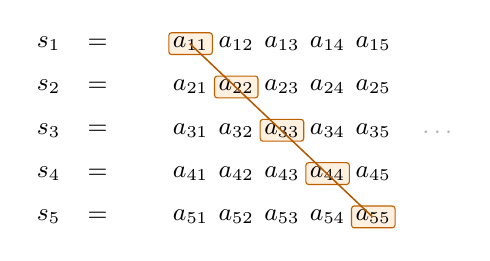
\begin{tikzpicture}[
  every node/.style={font=\small},
  digit/.style={font=\small},
  diagonal/.style={draw=orange!75!black, fill=orange!12, rounded corners=1pt, inner sep=1.5pt},
  guide/.style={orange!70!black, line width=0.55pt}
]
  \foreach \row/\name in {1/s_1,2/s_2,3/s_3,4/s_4,5/s_5} {
    \node[anchor=east] at (0,-0.55*\row) {$\name$};
    \node at (0.35,-0.55*\row) {$=$};
  }

  \foreach \row in {1,...,5} {
    \foreach \col in {1,...,5} {
      \node[digit] at (0.95+0.58*\col,-0.55*\row) {$a_{\row\col}$};
    }
  }

  \foreach \row in {1,...,5} {
    \node[diagonal] at (0.95+0.58*\row,-0.55*\row) {$a_{\row\row}$};
  }
  \draw[guide] (1.52,-0.55) -- (3.84,-2.75);

  \node[anchor=west, gray!60] at (4.35,-1.68) {$\cdots$};
\end{tikzpicture}

  \caption{Boxed entries $a_{nn}=s_n(n)$ whose bit flips define a sequence distinct from every listed row.}
  \label{fig:cantor-diagonal-binary-sequences}
\end{illustrationfigure}

Figure \ref{fig:cantor-diagonal-binary-sequences} marks the diagonal entries used in Theorem \ref{thm:binary-sequences-uncountable}.\\
Flipping the $n$th boxed bit forces $s(n)\neq s_n(n)$, so the constructed sequence cannot equal row $n$.


\subsection{Cardinal Comparison and the Continuum}

Throughout this subsection, assume Principle \ref{princ:axiom-of-choice-analysis} and use the initial-ordinal cardinality $\abs{X}$ from Definition \ref{def:cardinals-as-initial-ordinals}.

\begin{definition} \label{def:cardinal-comparison-and-arithmetic} \hlt{Cardinal Comparison and Arithmetic}\\
For sets $A,B$, define the \hlt{function set} by $A^B\defeq\{f\mid f:B\to A\}$. Let $\kappa,\lambda$ be cardinals.
\begin{enumerate}[label=(\roman*)]
\setlength{\itemsep}{0pt}
\item \hlt{Comparison}: the relations $\kappa\leq\lambda$ and $\kappa<\lambda$ are the corresponding ordinal comparisons.
\item The \hlt{cardinal sum} is $\kappa+\lambda\defeq\abs{(\{0\}\times\kappa)\cup(\{1\}\times\lambda)}$.
\item The \hlt{cardinal product} is $\kappa\lambda\defeq\abs{\kappa\times\lambda}$.
\item The \hlt{cardinal power} is $\kappa^\lambda\defeq\abs{\{f\mid f:\lambda\to\kappa\}}$.
\end{enumerate}
These are cardinal operations. Cardinal arguments distinguish them from the ordinal operations of Definition \ref{def:ordinal-arithmetic}.
\end{definition}

\begin{proposition} \label{prop:cardinal-operations-on-representatives} \hlt{Cardinal Comparison and Operations on Representatives}\\
Let $A,B$ be sets, and set $\kappa\defeq\abs{A}$ and $\lambda\defeq\abs{B}$.
\begin{enumerate}[label=(\roman*)]
\setlength{\itemsep}{0pt}
\item $\kappa\leq\lambda$ iff an injection $A\to B$ exists.
\item $\kappa<\lambda$ iff an injection $A\to B$ exists and $A\not\sim_{\#}B$.
\item $\kappa+\lambda=\abs{(\{0\}\times A)\cup(\{1\}\times B)}$. If $A\cap B=\emptyset$, then $\kappa+\lambda=\abs{A\cup B}$.
\item $\kappa\lambda=\abs{A\times B}$.
\item $\kappa^\lambda=\abs{A^B}$.
\end{enumerate}
\begin{proof}
Choose bijections $u:A\to\kappa$ and $v:B\to\lambda$ by Proposition \ref{prop:cardinality-canonical-and-bijection-invariant}(i).
\begin{enumerate}[label=(\roman*)]
\setlength{\itemsep}{0pt}
\item[$(i)$] ($\Rightarrow$) If $\kappa\leq\lambda$, then an injection $A\to B$ exists by Proposition \ref{prop:ordinal-cardinality-comparison}.
\item[$(i)$] ($\Leftarrow$) If an injection $A\to B$ exists, then $\kappa\leq\lambda$ by Proposition \ref{prop:ordinal-cardinality-comparison}.
\item[$(ii)$] ($\Rightarrow$) Suppose $\kappa<\lambda$. Then $\kappa\leq\lambda$ and $\kappa\neq\lambda$. An injection $A\to B$ exists by (i), and $A\not\sim_{\#}B$ by Proposition \ref{prop:cardinality-canonical-and-bijection-invariant}(ii).
\item[$(ii)$] ($\Leftarrow$) Suppose an injection $A\to B$ exists and $A\not\sim_{\#}B$. Then $\kappa\leq\lambda$ by (i) and $\kappa\neq\lambda$ by Proposition \ref{prop:cardinality-canonical-and-bijection-invariant}(ii), so $\kappa<\lambda$.
\item[$(iii)$] Set $U\defeq(\{0\}\times A)\cup(\{1\}\times B)$ and $V\defeq(\{0\}\times\kappa)\cup(\{1\}\times\lambda)$. Define $F:U\to V$ by $F(0,a)\defeq(0,u(a))$ and $F(1,b)\defeq(1,v(b))$.\\
The inverse sends $(0,\xi)$ to $(0,u^{-1}(\xi))$ and $(1,\eta)$ to $(1,v^{-1}(\eta))$, so $F$ is bijective by Theorem \ref{thm:bijective-iff-invertible-function}.\\
Hence $\abs{U}=\abs{V}$ by Proposition \ref{prop:cardinality-canonical-and-bijection-invariant}(ii), proving the first equality.\\
If $A\cap B=\emptyset$, define $G:U\to A\cup B$ by $G(0,a)\defeq a$ and $G(1,b)\defeq b$.\\
Its inverse sends $x\in A$ to $(0,x)$ and $x\in B$ to $(1,x)$, so $G$ is bijective. Thus $\kappa+\lambda=\abs{A\cup B}$ by Proposition \ref{prop:cardinality-canonical-and-bijection-invariant}(ii).
\item[$(iv)$] Define $P:A\times B\to\kappa\times\lambda$ by $P(a,b)\defeq(u(a),v(b))$. Its inverse is $(\xi,\eta)\mapsto(u^{-1}(\xi),v^{-1}(\eta))$, so $P$ is bijective by Theorem \ref{thm:bijective-iff-invertible-function}.\\
Therefore $\kappa\lambda=\abs{A\times B}$ by Proposition \ref{prop:cardinality-canonical-and-bijection-invariant}(ii).
\item[$(v)$] Define $T:A^B\to\{g\mid g:\lambda\to\kappa\}$ by $T(f)\defeq u\circ f\circ v^{-1}$. Its inverse sends $g:\lambda\to\kappa$ to $u^{-1}\circ g\circ v$, so $T$ is bijective by Theorem \ref{thm:bijective-iff-invertible-function}.\\
Hence $\kappa^\lambda=\abs{A^B}$ by Proposition \ref{prop:cardinality-canonical-and-bijection-invariant}(ii).
\end{enumerate}
\hlt{Structural Commentary}: Chosen bijections transport comparison and all three cardinal operations.\\
\hlt{Key Insight}: Bijections act coordinatewise on tags, pairs, and functions.
\end{proof}
\end{proposition}

\begin{definition} \label{def:continuum-cardinal} \hlt{Continuum Cardinal}\\
The \hlt{continuum cardinal} is $\mathfrak{c}\defeq2^{\aleph_0}$.
\end{definition}

\begin{proposition} \label{prop:continuum-cardinal-models} \hlt{Models of the Continuum Cardinal}\\
$\mathfrak{c}=\abs{\{0,1\}^{\N}}=\abs{\mathcal{P}(\N)}$.
\begin{proof}
The map $q:J_2\to\{0,1\}$ defined by $q(k)\defeq k-1$ is bijective. Thus $\abs{\{0,1\}}=2$ and $\abs{\N}=\aleph_0$ by Proposition \ref{prop:finite-cardinality-and-aleph-zero-agreement}(i),(iii).\\
Hence $\mathfrak{c}=\abs{\{0,1\}^{\N}}$ by Proposition \ref{prop:cardinal-operations-on-representatives}(v). The relation $\{0,1\}^{\N}\sim_{\#}\mathcal{P}(\N)$ holds by Proposition \ref{prop:binary-sequences-model-power-set}.\\
Hence $\abs{\{0,1\}^{\N}}=\abs{\mathcal{P}(\N)}$ by Proposition \ref{prop:cardinality-canonical-and-bijection-invariant}(ii).\\
\hlt{Structural Commentary}: Finite and countable representatives reduce cardinal exponentiation to binary functions and subsets.\\
\hlt{Key Insight}: A binary function is the characteristic function of one subset.
\end{proof}
\end{proposition}

\begin{corollary} \label{cor:continuum-strictly-exceeds-aleph-zero} \hlt{The Continuum Strictly Exceeds $\aleph_0$}\\
$\aleph_0<\mathfrak{c}$.
\begin{proof}
The map $j:\N\to\mathcal{P}(\N)$, $j(n)\defeq\{n\}$, is injective since $j(m)=j(n)\Rightarrow m=n$.\\
No bijection $\N\to\mathcal{P}(\N)$ exists by Theorem \ref{thm:cantor-power-set-theorem}. Therefore $\abs{\N}<\abs{\mathcal{P}(\N)}$ by Proposition \ref{prop:cardinal-operations-on-representatives}(ii).\\
The identities $\abs{\N}=\aleph_0$ and $\abs{\mathcal{P}(\N)}=\mathfrak{c}$ hold by Proposition \ref{prop:finite-cardinality-and-aleph-zero-agreement}(iii) and Proposition \ref{prop:continuum-cardinal-models}, respectively. Hence $\aleph_0<\mathfrak{c}$.\\
\hlt{Structural Commentary}: Singleton embedding gives weak comparison, while Cantor's theorem rules out equality.\\
\hlt{Key Insight}: The diagonal obstruction makes the continuum strictly larger.
\end{proof}
\end{corollary}


\subsection{Cardinal Arithmetic}

Throughout this subsection, assume Principle \ref{princ:axiom-of-choice-analysis} and use the cardinal operations from Definition \ref{def:cardinal-comparison-and-arithmetic}.

\begin{proposition} \label{prop:cardinal-arithmetic-reference-laws} \hlt{Cardinal Arithmetic Reference Laws}\\
Let $\kappa,\lambda,\mu$ be cardinals.
\begin{enumerate}[label=(\roman*)]
\setlength{\itemsep}{0pt}
\item $\kappa+\lambda=\lambda+\kappa$ and $\kappa\lambda=\lambda\kappa$.
\item $\kappa+(\lambda+\mu)=(\kappa+\lambda)+\mu$ and $\kappa(\lambda\mu)=(\kappa\lambda)\mu$.
\item $\kappa(\lambda+\mu)=\kappa\lambda+\kappa\mu$.
\item $\kappa^{\lambda+\mu}=\kappa^\lambda\kappa^\mu$, $(\kappa^\lambda)^\mu=\kappa^{\lambda\mu}$, and $(\kappa\lambda)^\mu=\kappa^\mu\lambda^\mu$.
\end{enumerate}
\begin{proof}
Set $A\defeq\{0\}\times\kappa$, $B\defeq\{1\}\times\lambda$, and $C\defeq\{2\}\times\mu$.\\
The sets are pairwise disjoint, and their coordinate projections are bijections onto $\kappa,\lambda,\mu$, respectively.\\
Thus $\abs{A}=\kappa$, $\abs{B}=\lambda$, and $\abs{C}=\mu$ by Proposition \ref{prop:cardinality-canonical-and-bijection-invariant}(ii) and Definition \ref{def:cardinals-as-initial-ordinals}.
\begin{enumerate}[label=(\roman*)]
\setlength{\itemsep}{0pt}
\item The identity is a bijection $A\cup B\to B\cup A$. The map $(a,b)\mapsto(b,a)$ is a bijection $A\times B\to B\times A$ with itself as inverse.
\item The equality $A\cup(B\cup C)=(A\cup B)\cup C$ holds.\\
The map $(a,(b,c))\mapsto((a,b),c)$ is a bijection $A\times(B\times C)\to(A\times B)\times C$ with inverse $((a,b),c)\mapsto(a,(b,c))$.
\item The equality $A\times(B\cup C)=(A\times B)\cup(A\times C)$ holds. The union on the right is disjoint because $B\cap C=\emptyset$.
\item Define $R:A^{B\cup C}\to A^B\times A^C$ by $R(f)\defeq(f|_B,f|_C)$. Its inverse is $R^{-1}(g,h)\defeq g\cup h$; disjointness makes this union a function.\\
Define $Q:(A^B)^C\to A^{B\times C}$ by $Q(F)(b,c)\defeq F(c)(b)$. Its inverse sends $h$ to $c\mapsto(b\mapsto h(b,c))$. Let $\pi_A(a,b)\defeq a$ and $\pi_B(a,b)\defeq b$.\\
The map $D:(A\times B)^C\to A^C\times B^C$ defined by $D(h)\defeq(\pi_A\circ h,\pi_B\circ h)$ has inverse $D^{-1}(f,g)(c)\defeq(f(c),g(c))$.
\end{enumerate}
Claims (i)--(iv) follow from these set equalities and bijections by Proposition \ref{prop:cardinal-operations-on-representatives}(iii)--(v).\\
\hlt{Structural Commentary}: Set identities and explicit bijections transport representative arithmetic to cardinal laws.\\
\hlt{Key Insight}: Restriction, currying, and projections control the exponent laws.
\end{proof}
\end{proposition}

\begin{theorem} \label{thm:infinite-cardinal-square-law} \hlt{Infinite Cardinal Square Law}\\
If $\kappa$ is an infinite cardinal, then $\abs{\kappa\times\kappa}=\kappa$.
\begin{proof}
\begin{enumerate}[label=(\roman*)]
\setlength{\itemsep}{0pt}
\item \hlt{Induction setup}: For an ordinal $\alpha$, let $P(\alpha)$ mean that, if $\alpha$ is an infinite cardinal, then $\abs{\alpha\times\alpha}=\alpha$.\\
Fix an ordinal $\kappa$ and assume $(\forall\beta<\kappa)\,P(\beta)$. It suffices by Principle \ref{princ:ordinal-foundations}(ii) to prove $P(\kappa)$.\\
The assertion $P(\kappa)$ is vacuous unless $\kappa$ is an infinite cardinal, so assume that it is.
\item \hlt{Well-order construction}: Define $r:\kappa\times\kappa\to\kappa$ by $r(\xi,\eta)\defeq\max\{\xi,\eta\}$.\\
For $p=(\beta,\beta')$ and $q=(\gamma,\gamma')$ in $\kappa\times\kappa$, declare $p\prec q$ when the first applicable condition holds:
\begin{enumerate}[label=(\alph*)]
\setlength{\itemsep}{0pt}
\item $r(p)<r(q)$;
\item $r(p)=r(q)$ and $\beta<\gamma$;
\item $r(p)=r(q)$, $\beta=\gamma$, and $\beta'<\gamma'$.
\end{enumerate}
Put $p\preceq q$ iff $p=q$ or $p\prec q$. Ordinal comparison makes these clauses exhaustive for distinct pairs.\\
Comparison by the first differing entry of $(r(p),\beta,\beta')$ is transitive and antisymmetric; hence $\preceq$ is a total order.\\
If $\emptyset\neq S\subseteq\kappa\times\kappa$, set $R_S\defeq\{r(p):p\in S\}$. The nonempty set $R_S$ has a least element $\rho$ by Principle \ref{princ:ordinal-foundations}(i).\\
Set $I_S\defeq\{\xi<\kappa:(\exists\eta<\kappa)\,[(\xi,\eta)\in S\land r(\xi,\eta)=\rho]\}$; it is nonempty by the definition of $\rho$.\\
The minimum $\xi_0\defeq\min I_S$ exists by Principle \ref{princ:ordinal-foundations}(i).\\
Set $J_S\defeq\{\eta<\kappa:(\xi_0,\eta)\in S\land r(\xi_0,\eta)=\rho\}$; it is nonempty by the definition of $I_S$.\\
The minimum $\eta_0\defeq\min J_S$ exists by Principle \ref{princ:ordinal-foundations}(i). Then $(\xi_0,\eta_0)$ is least in $S$, so $\preceq$ is a well-order.
\item \hlt{Ordinal comparison}: Choose an ordinal $\delta$ and an order isomorphism $f:(\delta,\leq)\to(\kappa\times\kappa,\preceq)$ by Principle \ref{princ:ordinal-foundations}(iii).\\
The map $\xi\mapsto(\xi,0)$ injects $\kappa$ into $\kappa\times\kappa$. Since $\abs{\kappa}=\kappa$ by Definition \ref{def:cardinals-as-initial-ordinals}, $\kappa\leq\abs{\kappa\times\kappa}$ by Proposition \ref{prop:ordinal-cardinality-comparison}.\\
The equality $\abs{\kappa\times\kappa}=\abs{\delta}$ holds by Proposition \ref{prop:cardinality-canonical-and-bijection-invariant}(ii), and $\abs{\delta}\leq\delta$ by Definition \ref{def:cardinals-as-initial-ordinals}. Thus $\kappa\leq\abs{\kappa\times\kappa}=\abs{\delta}\leq\delta$.
\item \hlt{Initial-segment contradiction}: Suppose $\kappa<\delta$. Write $f(\kappa)=(\beta,\beta')$ and set $X\defeq\{q\in\kappa\times\kappa:q\prec(\beta,\beta')\}$.\\
The restriction $f|_{\kappa}:\kappa\to X$ is bijective because $f$ preserves and reflects order.\\
Hence $\abs{X}=\kappa$ by Proposition \ref{prop:cardinality-canonical-and-bijection-invariant}(ii) and Definition \ref{def:cardinals-as-initial-ordinals}.\\
Set $\alpha\defeq\max\{\beta,\beta'\}+1$. Since $\beta,\beta'<\kappa$ and $\kappa$ is a limit ordinal by Lemma \ref{lem:infinite-cardinals-are-limit-ordinals}, $\alpha<\kappa$.\\
Set $\lambda\defeq\abs{\alpha}$. Then $\lambda$ is a cardinal, and a bijection $u:\alpha\to\lambda$ exists by Proposition \ref{prop:cardinality-canonical-and-bijection-invariant}(i).\\
Since $\lambda\leq\alpha$ by Definition \ref{def:cardinals-as-initial-ordinals}, $\lambda<\kappa$. If $q\in X$, then $r(q)\leq\max\{\beta,\beta'\}<\alpha$, so $q\in\alpha\times\alpha$.\\
The coordinate map $(\xi,\eta)\mapsto(u(\xi),u(\eta))$ is a bijection $\alpha\times\alpha\to\lambda\times\lambda$, whose restriction to $X$ is injective.\\
Thus $\kappa=\abs{X}\leq\abs{\lambda\times\lambda}$ by Proposition \ref{prop:ordinal-cardinality-comparison}. If $\lambda$ is finite, then $\abs{\lambda\times\lambda}<\aleph_0\leq\kappa$ by Theorem \ref{thm:multiplication-principle-finite-products} and Proposition \ref{prop:finite-cardinality-and-aleph-zero-agreement}.\\
If $\lambda$ is infinite, then $\abs{\lambda\times\lambda}=\lambda<\kappa$ by induction hypothesis. In either case, $\abs{\lambda\times\lambda}<\kappa$, contradicting $\kappa\leq\abs{\lambda\times\lambda}$; hence $\kappa\not<\delta$.
\item \hlt{Conclusion}: Since $\kappa\leq\delta$, $\delta=\kappa$ by Principle \ref{princ:ordinal-foundations}(i). Thus $f$ is a bijection $\kappa\to\kappa\times\kappa$, so $\abs{\kappa\times\kappa}=\kappa$ by Proposition \ref{prop:cardinality-canonical-and-bijection-invariant}(ii) and Definition \ref{def:cardinals-as-initial-ordinals}. Hence $P(\kappa)$ holds, completing the induction.
\end{enumerate}
\hlt{Structural Commentary}: Strong induction bounds max-ranked initial segments by smaller cardinal squares.\\
\hlt{Key Insight}: Every predecessor lies in a square of smaller cardinality.
\end{proof}
\end{theorem}

\begin{theorem} \label{thm:infinite-cardinal-absorption-reference} \hlt{Infinite Cardinal Absorption}\\
Let $\kappa,\lambda$ be cardinals, and let $\mu\defeq\max\{\kappa,\lambda\}$ be infinite.
\begin{enumerate}[label=(\roman*)]
\setlength{\itemsep}{0pt}
\item $\kappa+\lambda=\mu$.
\item If $\kappa,\lambda>0$, then $\kappa\lambda=\mu$.
\item $\aleph_0+\aleph_0=\aleph_0\aleph_0=\aleph_0$.
\end{enumerate}
\begin{proof}
The equality $\abs{\mu\times\mu}=\mu$ holds by Theorem \ref{thm:infinite-cardinal-square-law}. Set $U\defeq(\{0\}\times\mu)\cup(\{1\}\times\mu)$.\\
Since $0,1\in\mu$, the maps $\xi\mapsto(0,\xi)$ and $(i,\xi)\mapsto(\xi,i)$ inject $\mu$ into $U$ and $U$ into $\mu\times\mu$, respectively.\\
The identities $\abs{U}=\mu+\mu$ and $\abs{\mu}=\mu$ hold by Definition \ref{def:cardinal-comparison-and-arithmetic} and Definition \ref{def:cardinals-as-initial-ordinals}, respectively.\\
Thus $\mu\leq\mu+\mu\leq\abs{\mu\times\mu}=\mu$ by Proposition \ref{prop:ordinal-cardinality-comparison}, so $\mu+\mu=\mu$.
\begin{enumerate}[label=(\roman*)]
\setlength{\itemsep}{0pt}
\item Set $V\defeq(\{0\}\times\kappa)\cup(\{1\}\times\lambda)$. If $\mu=\kappa$, then $\xi\mapsto(0,\xi)$ injects $\mu$ into $V$; if $\mu=\lambda$, then $\xi\mapsto(1,\xi)$ does so.\\
The inclusions $\kappa\hookrightarrow\mu$ and $\lambda\hookrightarrow\mu$ induce an injection $V\to U$, and $\abs{V}=\kappa+\lambda$ by Definition \ref{def:cardinal-comparison-and-arithmetic}.\\
Thus $\mu\leq\kappa+\lambda\leq\mu+\mu=\mu$ by Proposition \ref{prop:ordinal-cardinality-comparison}, so $\kappa+\lambda=\mu$.
\item Assume $\kappa,\lambda>0$, so $0\in\kappa\cap\lambda$. If $\mu=\kappa$, then $\xi\mapsto(\xi,0)$ injects $\mu$ into $\kappa\times\lambda$; if $\mu=\lambda$, then $\xi\mapsto(0,\xi)$ does so.\\
The coordinate inclusions induce an injection $\kappa\times\lambda\to\mu\times\mu$, and $\kappa\lambda=\abs{\kappa\times\lambda}$ by Definition \ref{def:cardinal-comparison-and-arithmetic}.\\
Thus $\mu\leq\kappa\lambda\leq\abs{\mu\times\mu}=\mu$ by Proposition \ref{prop:ordinal-cardinality-comparison}, so $\kappa\lambda=\mu$.
\item The cardinal $\aleph_0$ is infinite by Proposition \ref{prop:finite-cardinality-and-aleph-zero-agreement}(iv). The asserted equalities follow by (i),(ii) with $\kappa=\lambda=\aleph_0$.
\end{enumerate}
\hlt{Structural Commentary}: The square law sandwiches each sum and nonzero product between $\mu$ and itself.\\
\hlt{Key Insight}: An infinite maximum absorbs every bounded factor.
\end{proof}
\end{theorem}

